\section{Gleichstrommaschinen (GSM)}
    \subsection{Funktionsprinzip}
    Ein Gleichstrom ist durchfliesst ein Schleife, welche sich in einem Magnetfeld befindet. \\
    Durch die Lorenzkraft wirkt auf die Schleife ein Drehmoment, welche sie in eine maximal halbe Drehung versetzt.
    Danach muss man den Schleifenstrom umpolisieren, um die Drehung weiter zu führen. \\
    \abb{images/GSM_Funktion.png}{14cm}{Funktion eines GSM mit Stromwender}
    \abb{images/GSM_Ersatz.png}{14cm}{Erstzschema der 4 Schaltungsarten}
    \textbf{A1-A2:} Ankerwicklung, \textbf{B1-B2:} Wendepolwicklung, \textbf{C1-C2:} Kompensationswicklung, \\
    \textbf{D1-D2:} Reihenschlusswicklung, \textbf{E1-E2:} Nebenschlusswicklung, \textbf{F1-F2:} Fremderregte Wicklung \\
    \begin{figure}
	    \centering
	    \begin{subfigure}[t]{0.45\textwidth}
	    	\centering
	    	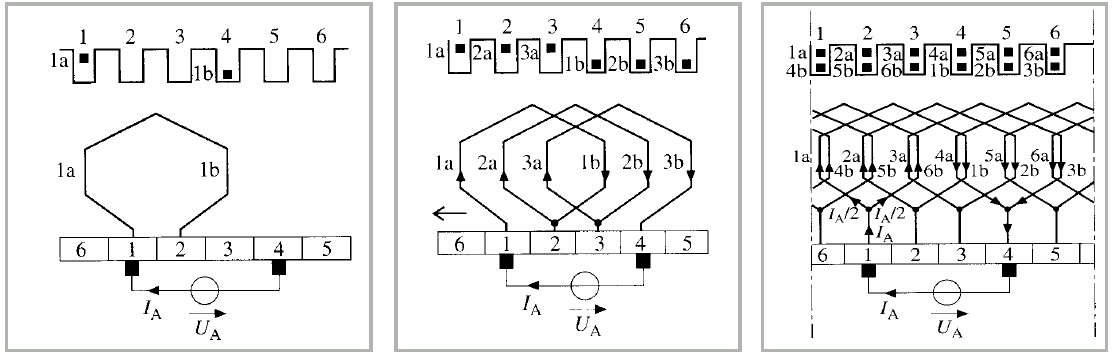
\includegraphics[width=\textwidth]{images/GSM_Wicklungen.png}
	    	\caption{Entstehung einer Schleifenwicklung}
	    \end{subfigure}
	    \begin{subfigure}[t]{0.45\textwidth}
	    	\centering
	    	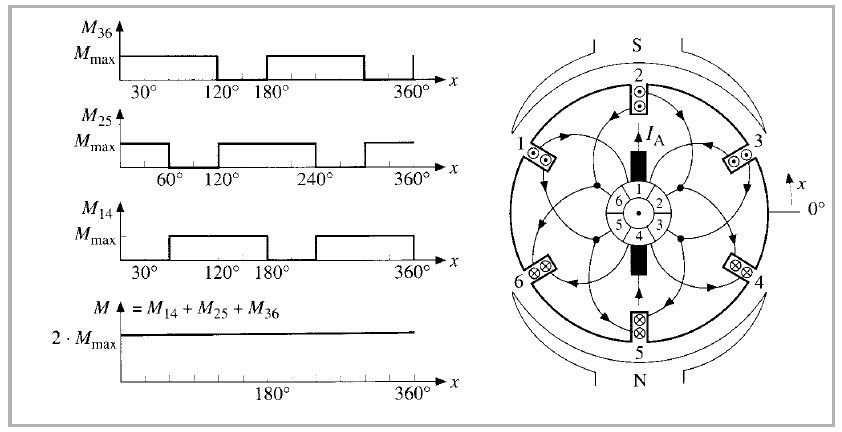
\includegraphics[width=\textwidth]{images/GSM_Drehmomentdarstellung.png}
	    	\caption{Alle Drehmomente zusammen ergeben ein gleichmässiges Drehmoment}
	    \end{subfigure}
    \end{figure}

    
    \subsection{Grundgleichungen}
    \begin{tabular}[c]{ | p{6cm} | p{9cm} |}
    	\hline
    	Umfangsgeschwindigkeit & $v_u=\omega\cdot R = 2\pi\cdot n \cdot
    	R=\frac{2\pi\cdot f \cdot R}{p}=2\cdot f \cdot \tau_p = d\cdot\pi\cdot n$\\
    	 & Geometrisch: $v=d\cdot\pi\cdot f$\\
    	\hline
    	Teilspannung eines Leiters & $U_{iL}=2\cdot \tau_p \cdot f \cdot l \cdot
    	B_m= 2\cdot f\cdot \Phi = 2\cdot p \cdot n \cdot \Phi$\\
    	\hline
    	Gesamtspannung & $U_i=\frac{z}{2\cdot a}\cdot U_{iL}=\frac{z}{a}\cdot
    	p \cdot n \cdot \Phi=k_1\cdot\Phi\cdot n = B_m \cdot z \cdot l \cdot v$\\
    	\hline
    	Ankerspannung & $U_a=R_a\cdot I_a + L_a\frac{dI_a}{dt}+U_i = U_i + U_{BK} + I_{AN} \cdot R_A$ \\
    	\hline
    	Erregerspannung & $U_e=R_e\cdot I_e + L_e\frac{dI_e}{dt}$\\
    	\hline
    	Induzierte Spannung & $U_i = k_1\cdot \Phi \cdot \omega_{mech} = B\cdot l
    	\cdot v \quad k_1 = Maschinenkonstante$\\
    	\hline
    	& $M_{el}=M_{Welle}+M_{Reibung}+J\cdot\frac{d\omega_{mech}}{dt}=k_1\cdot
    	\Phi\cdot I_a$\\
    	\hline
    	& $\Phi = \frac{L_e}{N_e}\cdot I_e$\\
    	\hline
    	Ideale Luftspaltleistung & 
    		$P_{Luft}=U_i\cdot I_A = M_{Luft} \cdot \omega $\\
    	\hline
    	Ideales Luftspaltderhmoment & 
    		$M_{Luft} = N \cdot B \cdot I \cdot d \cdot l$ \\
    	\hline
    	Mech. Leistung an der Welle &
    	$P_{Welle}=P_{Luft}-V_{Fe}-V_{Reib}-V_{zus}$\\
    	\hline
    	
    
    \end{tabular}
    
    \subsection{Nebenschluss Maschinen}
        \renewcommand{\arraystretch}{2}
        \begin{tabular}[c]{ | p{6cm} | p{9cm} |}
            \hline
            Drehzahl &
            $ n= \frac{U}{k_1 \cdot \Phi} - \frac{R_A \cdot M}{k_1 \cdot k_2 \cdot \Phi^2} \sim \frac{U}{I_E} - \frac{M}{I_E^2}$ \\ 
            &
            $\Longrightarrow $ bei $I_E$ = 0 und $M$ = 0 $n \rightarrow \infty$ \\
            \hline
            Drehmoment &
            $M=\frac{k_2 \cdot \Phi \cdot U_{Anker}}{R_{Anker}} - \frac{k_1 \cdot k_2 \cdot\phi^2 \cdot n}{R_A} =\frac{P_{mech}}{2\pi n_N}=\frac{U_{iN}I_N}{2\pi n_N}\sim I_E \cdot U_A - I_E ^2 \cdot n$ \\
            \hline
            Leistung &
            $P_{Anker}= U_i \cdot I \pm I^2 \cdot R_A $(+ bei Motor; - bei Generator) \\
            \hline
            Anlaufmoment &
            $M_A = \frac{k_1 \cdot \Phi \cdot U}{R_1}$ \\
            \hline
            Leerlaufmoment &
            $n_0 = \frac{U}{k_1 \cdot \Phi}$ \\
            \hline
            & $\Phi=\frac{L_e}{N_e}\cdot\frac{U_a}{R_e+R_v}$\\
            \hline
            Leerlaufdrehzahl &
            $\omega_m=\frac{N_e\left(R_E+R_V\right)}{k_1\cdot
            L_e}-\frac{R_a\left(R_e+R_V\right)^2N_e^2}{\left(k_1L_eU_a\right)^2}\cdot
            M_{el}$\\
            \hline
        \end{tabular}
        \renewcommand{\arraystretch}{1.5}
        
    \subsection{Reihenschluss Maschine}
    Auch bekannt als Seriemaschine oder Hauptschlussmaschine\\
        \renewcommand{\arraystretch}{2}
        \begin{tabular}[c]{ | p{6cm} | p{9cm} |}
            \hline
            Drehmoment &
            $ M=  \frac{U_{Induziert} \cdot I_A}{2 \cdot \pi n_N} = \frac{k_1 \cdot k_E \cdot I_A ^2}{2\cdot \pi n_N}= \frac{k_1 \cdot k_E}{2 \cdot \pi n_N}\cdot(\frac{U}{R_A + R_E + k_1 \cdot k_E \cdot n})^2$ \\
            \hline
            Anlaufstrom &
            $I_A=\frac{U_N}{\sum R_a}=\frac{U_N I_N^2}{U_N I-P_N}$ \\
            \hline
            & $M_{el}=\frac{L_e}{N_e}k_1\cdot I_a^2$\\
            \hline
            Leerlaufdrehzahl &
            $\omega_m=\frac{N_e}{L_e}\frac{U_a}{k_1I_a}-\frac{N_e}{L_e}\frac{R_a+R_e}{k_1}=\frac{\sqrt{N_e}\cdot
            U_a}{\sqrt{L_ek_1M_{el}}}-\frac{N_e}{L_e}\frac{R_a+R_e}{k_1}$\\
            \hline
        \end{tabular}
        \renewcommand{\arraystretch}{1.5}